%%%%%%%%%%%%%%%%%%%%%%%%%%%%%%%%%%%%%%%%%%%%%%%%%%%%%%%%%%%%%%%%%%%%%%%%%%%%%%%%%%%%%%%%%%%%%%%%%%%%%%
%
%   Filename    : chapter_1.tex 
%
%   Description : This file will contain your Research Description.
%                 
%%%%%%%%%%%%%%%%%%%%%%%%%%%%%%%%%%%%%%%%%%%%%%%%%%%%%%%%%%%%%%%%%%%%%%%%%%%%%%%%%%%%%%%%%%%%%%%%%%%%%%

%added by sir jd just for fun
\epigraph{Music is a science which must have determined rules. These rules must be drawn from a principle which should be evident, and this principle cannot be known without the help of mathematics. I must confess that in spite of all the experience which I have acquired in music by practicing it for a fairly long period, it is nevertheless only with the help of mathematics that my ideas became disentangled and that light has succeeded to a certain darkness of which I was not aware before.}{\textit{\citep{rameau1722traite}}}


\chapter{Research Description}
\label{sec:researchdesc}    %--note: labels help you with hyperlink editing (using your IDE)

 
\section{Overview of the Current State of Technology}
\label{sec:overview}

%Paragraph 1
Music has been known to be an effective learning companion for children \cite{mcintire2007developing}. 
It is an integral part of their lives helping them understand the different complexities of life. Several applications and technologies have been developed to help children throughout their learning journey \cite{roschelle2000changing}.

%Paragraph 2
Music can trigger many types of memories in children and can be used to engage with them at any time. This makes music play an important role in their education \cite{levinowitz1999importance}. On the other hand, computers and digital applications have become part of a child's daily life which can lead the child to be more productive in doing educational tasks. By utilizing these technologies, music can contribute towards the overall learning of the child in certain knowledge areas like science and mathematics \cite{zaranis2013using}.

%Paragraph 3
%music is a difficult field of study
Music is also a complex cultural phenomena making it difficult to study as it has a wide variety of theories to learn \cite{byrd2009studying}. 
%why is music difficult
One of the main reasons that makes it difficult is its many representations. Since music is considered as a form of art, composers have the freedom to make music in any way so that they can define it the way they want it to be \cite{byrd2009studying}. 

%Paragraph 4
The difficulty in teaching a child to learn music is on how to make it enjoyable for them, as the learning comes from them exploring various instruments at an early age \cite{ghazali2005minds}. This playful nature leads to them doing simple acts like singing and playing musical games which can serve as a foundation in giving them a basic idea on musical theories. Copying or repeating sound, enables children to learn from different sound sources, giving them a sense of some musical rudiments like rhythm and pitch \cite{mcpherson2015child}. 


%Paragraph 5
%name specific studies/systems for teaching music or mobile music or learning with music (name 2-3 siguro)-=][=--]
Multimedia Technology has been widely used in the education of students especially in the field of teaching music \cite{tong2016design}. Examples of these technologies include applications such as Musilla Musical School \cite{educationalappstore2017}, which is an application designed to teach the principles of music to children. Another is Sesame Street Makes Music \cite{educationalappstore2015}, which is an application designed to help children explore instruments, tempo, and musical creativity. However these applications pose further opportunities for lurning such as the limitations in accurate representations.
% However these applications have some gaps in the education such as the Musilla Musical School having a  thoroughly planned curriculum and some inaccurate representations of key musical concepts such as rhythm and melody. The Sesame Street Makes Music also has its gaps by having a limited song choice. (@mart Comment ni sir baka pwede ilagay yung gaps ng 2 apps na to sa rrl)

%http://journals.sfu.ca/onlinejour/index.php/i-jet/article/view/5686
% first app: https://www.educationalappstore.com/app/mussila-music-school
%second app: https://www.educationalappstore.com/app/sesame-street-makes-music

%Paragraph 6
%Guide ni sir:
%Teka baket sandbox bigla haha sana may discussion muna on samples of these approaches such as mnemonic, instructional and while some follow the sandbox approach….
There are many different approaches that help in learning. One common way is children attending traditional schools as they use the instructional approach of learning where there is a teacher guiding them throughout the process. Another approach which is mostly unconventional in schools is the use of mnemonics where relatable associations are used to remember complpex ideas \cite{putnam2015mnemonics}. Next is the sandbox approach where the child can playfully learn using a virtual sandbox environment on their own. Here, they discover by themselves the ideas by exploring and playing around the sandbox environment. We want to discover whether these technologies such as implementing a virtual sandbox environment can enable children to play, create and explore music.

%Paragraph 7
%what is the sandbox approach?
%what makes it sandbox environemnet
%name some notable learning sandbox environment: (use Scratch.... then cite niyo na paper nila Giselle)
%sandbox for math, sandbox for machine learning... other sandbox
The sandbox approach is implemented usually in a specific software platform. This provides control over the resources that the software or users can use \cite{prevelakis2001sandboxing}. Much like the literal sandbox where people can only use items inside it, such an environment allows users to only interact with what is provided to them \cite{goldberg1996secure}. An example of a notable learning sandbox environment is Scratch
% (cite scratch paper)
. It is a visual programming language developed to deal with the problem of learning programming for novices, especially younger users \cite{maloney2010scratch}. It uses the sandbox approach to assist young people learn how to think creatively, reason systematically \cite{kaleliouglu2014effects}.
Its implementation of the sandbox approach aids children in learning how to work successfully with others, and think ingeniously \cite{nodalo2019building}. Another notable learning sandbox environment is the Sonification Sandbox \cite{walker2003sonification}. It allows users to independently map several data sets to timbre, pitch, volume, and pan, with full control over the default, minimum, maximum, and polarity for each attribute \cite{walker2003sonification}. By using the features from Sonification Sandbox, we get to take advantage of these features.


%Paragraph 8
%meron bang sandbox for music?
%two options
% option1: there are. if there are discuss their gaps, and areas for improvement
% option2: if wala, or limited... then we have we want to discover if we can introduce the sandbox approach
%we mention Otomushi, what about otomushi?
OtoMushi, derived from its Japanese meaning where \textit{oto} means sound and \textit{mushi} means insect, is a platform for interacting with sound samples which is represented by insects developed by Andre (2010). Its sandbox environment allows a controlled canvass where users can mix virtual creatures applying scratching techniques to explore sound \cite{andre2010otomushi}. It allows users to record sound when they speak. A tangible sandbox environment surface called smartskin by \cite{rekimoto2002smartskin} lacked responsiveness and that the resolution of the graphics were bad. In later iterations, OtoMushi was implemented on the iPad. By implementing it this way, children can play with the tool as if it was a virtual sandbox environment. With this, a child's playfulness can be exploited by allowing them to play with the tool as much as they want.
%  This makes it prone to noise and static sounds which makes it ineffective.
% 音虫

%Paragraph 9
%what is our RQ?
%(RQ)How might we design a sandbox environment and a firefly model that will help children learn music in a playful manner
%objective general objective: This research aims to answer the following research question?
    Music has many complex properties that make it difficult to learn. Children are also difficult to teach because they have a shorter attention span and require many repetitions when teaching music \cite{may2013public}. Sandbox environments have been found to work on children since play is central to early childhood education and it also provides a safe yet playful environment suited for their learning \cite{bos2014learning, dalgarno2010learning}. There are many music applications across several platforms that help in teaching music to children but there are only few that incorporate a sandbox environment that helps in accompanying their learning. With all these the tools and environments, this study aims to delve into the design of an interaction that will help children learn through a playful mobile interface.

%--- the following example shows how to include a figure in PNG format
% \begin{figure}[t]                %-- use [t] to place figure at top, [b] to place at the bottom, [h] for here
%   \centering                    %-- use this to center the figure
%   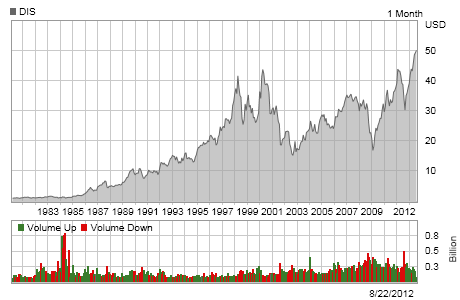
\includegraphics{DisneyChart.png}      %-- include image file named as "disneychart.png" 
%   \caption{This is the figure's caption -- Disney stock chart}
%     \label{fig:disneystock}
% \end{figure}


%
% Examples:
%     	Smith (1970) compared reaction times . . .
%     	In a recent study of reaction times (Smith, 1970), . . .   
%     	In 1970, Smith compared reaction times . . .
%	Smith, et al., (1970) compared reaction times . . .
%     	In a recent study of reaction times (Smith, et al., 1970), . . .  
%     	In 1970, Smith, et al., compared reaction times . . .
%

% Here are some examples on how to do the referencing (note author's name and years are different
% from commented examples).  For APA citation details, refer
% to \url{http://www.ctan.org/tex-archive/biblio/bibtex/contrib/apacite/}. 

% \begin{itemize}
%  \item \citeA{kartch:2000:ERA} compared reaction times...
%  \item In a recent study of reaction times \cite{kartch:2000:ERA}...
%  \item In \citeyearNP{kartch:2000:ERA}, \citeauthor{kartch:2000:ERA} compared reaction times...
%  \item \shortciteA{fedkiw:2001:VSO} compared reaction times... 
%  \item In a recent study of reaction times \cite{fedkiw:2001:VSO}...
%  \item In \citeyearNP{fedkiw:2001:VSO}, \shortciteauthor{fedkiw:2001:VSO}, compared reaction times...
% \end{itemize}

% The following are references from journal articles \cite{Park:2006:DSI, Pellacini:2005:LAH, 
% sako:2001:SSB}.  Here's an MS thesis document \cite{yee:2000:SSA}, and this is from
% PhD dissertation \cite{kartch:2000:ERA}. For a book, reference is given as 
% \cite{parke:1996:CFA}.  Proceedings from a conference samples are \cite{Jobs95, fedkiw:2001:VSO,
% levoy:2000:TDM}.  The sample bibliography file named \textbf{myreferences.bib} is from the
% SIGGRAPH \LaTeX template.  You can use a text editor to view the contents of the bib file.  
% It is your task to create your own bibliography file.  For those who downloaded papers from
% ACM or IEEE sites, there is a BibTeX link that you can click; thereafte   r, you just simply need
% to copy and paste the BibTeX entry into your own bibliography file.



% The following shows how to include a program source code (or algorithm).  The verbatim environment,
% as the name suggests, outputs text (including white spaces) as is...

% \begin{verbatim}
%               #include <stdio.h>
%               main()
%               {
%                     printf("Hello world!\n");
%               }
% \end{verbatim}


% \textcolor{red}{DO NOT FORGET to write the statement of the research problem here, i.e.,
% before the Research Objectives.}


\section{Research Objectives}
\label{sec:researchobjectives}

\subsection{General Objective}
\label{sec:generalobjective}

% To design a sandbox environment and a firefly model which is a firefly with different parts that represent different musical elements that will help children learn music in a playful manner.

This study aims to identify and model the human factors and behaviours that children exhibit when given the task of learning how to compose music with a mobile musical tool.

\subsection{Specific Objectives}
\label{sec:specificobjectives}

%
%  \begin{comment} ... \end{comment} is used for multiple lines of comment
%

\begin{comment}

This subsection is an elaboration of the general objective.  It states the specific steps that must be undertaken to accomplish the
general objective.  These objectives must be specific, measurable, attainable, realistic, time-bounded.  Each specific objective may
start with ``to design/survey/review/analyze''

Studying a particular programming language or development tool (e.g., to study Windows/Object-Oriented/Graphics/C++ programming) to 
accomplish the general objective is inherent in all thesis and, therefore, must not be included here.


%
% IPR acknowledgement: the following sentences and examples are from Ethel Ong's slides 
%     on Research Objectives
%

How to formulate your research objectives:
1. Identify what research steps do you need to perform to achieve your general objective.
2. Identify the questions that must be answered for you to achieve your general objective.
    Thereafter, convert these questions into action statements


Example #1:

Research Question:
  What are the general features of a web-based learning environment?

Specific Objective:
   To review existing web-based learning environment that teaches language learning for children


Example #2:

Research Question:
   How will you represent commonsense knowledge for use by computer systems?

Specific Objective:
   To identify knowledge representation approaches used by existing story generation systems

Example #3:
Research Question:
   What types of storytelling knowledge are needed to generate stories?

Specific Objective:
    To identify the different types of storytelling knowledge used in generating stories

Example #4:
Research Question:
    What machine learning approaches will you utilize?

Specific Objective:
    To determine existing machine learning algorithms [that can be used in training the computer system to detect cyberbullying cases] 

Example #5: Research Question:
    How will your research output be evaluated?

Specific Objective:
    To define evaluation metrics for validating the accuracy of the translation

\end{comment}

%
%  The following are example specific objectives; replace them with your own 
%
This research shall attempt to answer the following specific questions:
\begin{enumerate}
%   \item To design a sandbox environment where children can interact with firefly models.
%   \item To design a firefly model that will represent musical features playable by children.
%   \item To integrate the sandbox environment and firefly model in a mobile application.
%     \item To evaluate the usability of the sandbox environment, and the firefly models in terms of helping children learn music.
\item What activities do music teachers implement when teaching children music patterns?
\item What features can be designed to enable playful interactions when teaching children music?
\item What human factors do children exhibit when using the firefly and sandbox model?
\end{enumerate}


\section{Scope and Limitations of the Research}
\label{sec:scopelimitations}

    FireflyX is a virtual mobile music environment that will be developed on the iOS platform as a tablet application. With the use of the application, children can create their own music in an environment without the fear of breaking anything. The canvas will be able to house up to 5 virtual firefly models which can simultaneously produce sound making the environment multi-melodic when they are released. It will only provide what is needed by the children namely starting the composition, composing the rhythm,pitch and tempo by configuring the firefly model, and playing the composition in the environment with the other created fireflies. We would be observing the children based on how they are taught musical theories and our research will include students from different schools and their music classes.
    
    The firefly model will have a set musical features attached to its corresponding parts. These “movable” parts include the body, wings, and tail. Through the different parts of the firefly, children can configure the music through the use of interchangeable firefly model parts. These parts represent different musical rudiments of rhythm like clap-rest pattern, speed of sustain, and number of repetitions. It will also represent pitch and tempo as well. The firefly model can also represent one instrument and the target instrument for music creation is the piano due to its popularity with children. One firefly will represent one layer of the rhythm, pitch and tempo also for this model music filters will not be included. Dotted notation will not be included as well. The 4/4 time signature will only be the used by all firefly models. When the children are done manipulating the parts of the firefly model, the firefly model is released and the sound is created by the combination of the parts is played.
    
    The interactions the children will be limited to touch gestures that the mobile platforms can handle. Several touch gestures will be incorporated in the design to enable the children to play with the virtual firefly model. Such gestures include tap, drag, swipe, and flick. The target users of the application are children from ages 5-8. To evaluate the usability of the application the group will be evaluating the learning of children by giving them a set of instructions. After giving the instructions, we will be asking the music expert to evaluate the performance of the child. We will also be observing children use the app and assess the app’s usability afterwards.

\begin{comment}

%
% IPR acknowledgement: the sentences inside this comment are from Ethel Ong's slides on Scope and Limitations of the Research
%
Generally, one paragraph should be allotted for each of your research objectives.

Each paragraph contains a brief overview of the concept/theory and the purpose of doing the associated objective.

Each paragraph also includes a description of the scope/limitation of your study.

* Please refer to the slides for examples.

\end{comment}
    

\section{Significance of the Research}
\label{sec:significance}

This study attempts to design a usable mobile musical learning tool for children that incorporates computer-aided creativity, music elements and many others which can help children users to learn music theories at a young age. Additionally, the function of this tool will contribute in creating a child friendly interface for children to learn a hard concept like music. 

This tool will help children learn music through the sandbox interface that the application presents. The study helps to offer other music application developers an idea on how to design sandbox environments and integrate them into music learning.

Development of tools like this would give a basis for instructional designers to develop mobile products on what to do and what not to do when designing and developing these kinds of applications. What this study can offer can be set as a benchmark on what the quality of these products when they will release onto the public would be.

%
% IPR acknowledgement: the following list of items are from Ethel Ong's slides on Significance of the Research
%
% \begin{itemize}
% \item  What is the relevance of your work to the computer science community? 

% \begin{itemize} 
% \item What will be your technical contributions, in terms of algorithms, or approaches, or new domain? 
% \item What is your value-added compared to existing systems? 
% \end{itemize}

% \item What will be your contributions to society in general? 
%     \begin{itemize}
%       \item Who will benefit from your system? 
%       \item Who are your target users and how will this system benefit them? 
%   \end{itemize}
% \end{itemize}

% \begin{comment}
% If applicable, describe possible commercialization and/or innovation in your research.
% \end{comment}
\begin{comment}
\section{Research Methodology}
This chapter discusses the activities and specific steps that was done in this research. It also includes the the activities from thesis proposal to final thesis defense.

\subsection{Planning}
In this phase it shows the formulation of the thesis topic with the research problems and objectives, including the scope and limitation with the help of the thesis adviser. This also includes the planning of the future steps to do and what the output of the research is.

\subsection{Review of Related Literature}
Relevant works on Computer-Aided Instruction (CAI), Sandbox environments, and similar software's are being read and studied by the group to give the needed understanding to conduct the study. Works about Computer-Aided Instruction are important to the study as they provide an idea on how past applications have aided people in learning. Works on Sandbox environments will also be reviewed as they provide an idea on how we can implement the virtual environment that is suitable to the learning of the children and also how to test the usability of the said environment. Finally, works on similar software will also be reviewed to give context on how to make the tool usable and enjoyable for use of the children.

\subsection{Data Collection}
In this phase, the group will research on music theory and concepts. The information gathered there will be used for building the model for the musical representation of the tool. The group will also ask music experts on how to best evaluate children on their learning, as it is important to get their opinions on how to properly evaluate the children.

\subsection{Interaction Design}
This phase is concerned on building the experience that the users have with the application and listing down the steps on how it would help them. This part will also include on deciding on the user interface elements, and also how the users will interact with these elements. The data gathered from the group observing the users during testing will give good insight on what design elements we are good and what else we can improve on. The group will be making artifacts and user personas to represent the users, as this will be used in validating throughout different tests. All of these are to be done to make sure that we would integrate the solution to help in the learning of children. 

\subsection{Implementation}
In the implementation of the system, it will be a mobile application on the iOS platform. We chose IOS because IOS offers a less variety of screen sizes making it easier to design applications for. For the ease of use of the children it will be focused for the iPads, as it will be easier for them to interact with it due to iPads having a larger screen size than regular phones. As stated in the interaction design we will use the data gained from the observation throughout the different iterations of testing to further improve the implementation of the system.
    
\subsection{Testing}
To asses the effectiveness of the system that was developed, through out the research many iterations of testing will be done. These experiments will be designed to measure two things the first is the overall learning of the children and second is to measure the user experience and the interaction they have with it. We will use user experience metrics to help asses the overall experience. For the testing of the tool for the children we would ask help from a music expert to asses the children on their learning. The tests will be conducted throughout multiple weeks to see if the child is improving in his knowledge of music which will come from the feedback of the music expert. In every test that will be conducted they will be given a consent form, stating the ethical considerations of the research and they are given a chance to opt out during testing. All these are done to identify the issues that that iteration of the system has so that it can be improved upon.

\subsection{Results and Analysis}
This phase consists of analyzing the findings that were gathered during the different iterations of testing. Performing qualitative and quantitative analysis on the data that was gathered, also performing statistical treatment on the data. This is going to be used in deciding the features that will be improved on and to be added in the future. The creation of use cases and testing scenarios will be done in this stage. We will also follow the ethics in research as we would keep the data of the test subjects as confidential. Everything that was gathered will only be used for this research and they will not be shared or released to the public.

\subsection{Documentation}
Documentation will be done throughout the research. This will include all the documentation on all activities done including the results and analysis of each one. During testing the group will be documenting all events through note taking and video recording with the consent of the participants.

\subsection{Calendar of Activities}
Table \ref{tab:ganttChart} shows the Gantt chart of the activities done. Each bullet represents approximately one week worth of activity.


\begin{landscape}
\begin{table}[H]
\centering
\caption{Timetable of Activities} \vspace{0.25em}
\begin{tabular}{|l|l|l|l|l|l|l|l|l|l|l|l|l|l|l|l|l|}
    \hline
    2019 - 2020                  & May  & Jun   & July & Aug  & Sep & Oct & Nov & Dec & Jan  & Feb  & Mar  & Apr & May  & Jun  & Jul  & Aug \\ \hline
    Planning                     & \textbullet    & \textbullet     & \textbullet    & \textbullet    & ~   & ~   & ~   & ~   & ~    & ~    & ~    & ~   & ~    & ~    & ~    & ~   \\ \hline
    RRL & \textbullet\textbullet\textbullet\textbullet & \textbullet\textbullet\textbullet\textbullet & \textbullet\textbullet\textbullet\textbullet & \textbullet\textbullet\textbullet\textbullet & ~   & ~   & ~   & ~   & ~    & ~    & ~    & ~   & ~    & ~    & ~    & ~   \\ \hline
    Learning Swift      & ~    & ~     & \textbullet\textbullet\textbullet & \textbullet\textbullet\textbullet  & \textbullet\textbullet  & \textbullet   & \textbullet   & ~   & ~    & ~    & ~    & ~   & ~    & ~    & ~    & ~   \\ \hline
    Development                  & ~    & ~     & ~    & ~    & ~   & ~   & \textbullet   & \textbullet\textbullet  & \textbullet\textbullet\textbullet\textbullet & \textbullet\textbullet\textbullet\textbullet & \textbullet\textbullet\textbullet\textbullet & \textbullet\textbullet  & ~    & ~    & ~    & ~   \\ \hline
    Experiment Design              & ~    & ~     & ~    & ~    & ~   & ~   & ~   & ~   & ~    & \textbullet    & \textbullet\textbullet   & \textbullet\textbullet  & ~    & ~    & ~    & ~   \\ \hline
    Results and Analysis         & ~    & ~     & ~    & ~    & ~   & ~   & ~   & ~   & ~    & ~    & ~    & \textbullet\textbullet\textbullet & \textbullet\textbullet\textbullet\textbullet & \textbullet\textbullet\textbullet\textbullet & ~    & ~   \\ \hline
    Documentation                & \textbullet    & \textbullet     & \textbullet    & \textbullet    & \textbullet   & \textbullet   & \textbullet   & \textbullet   & \textbullet    & \textbullet    & \textbullet    & \textbullet   & \textbullet\textbullet   & \textbullet\textbullet\textbullet\textbullet & \textbullet\textbullet\textbullet\textbullet & \textbullet   \\ \hline
\end{tabular}
\label{tab:ganttChart}
\end{table}
\end{landscape}

\end{comment}
